
\section{General purpose algorithms}

We will start by introducing different proven properties for general purpose algorithms. These typically serve as primitives for many other algorithms and their study therefore provides a solid basis for dealing with more complex problems. It is therefore all the more important to have efficient algorithms for them.

\subsection{Scanning}

Scanning is the basic operation which consists simply in consulting each of the elements in a contiguous collection in memory. Naturally, its complexity is bounded by $O(\frac{N}{PB})$. The same applies if we run several scans in parallel, like reversing the input.

\subsection{Searching}

Searching for an item in a sorted collection benefits relatively little from parallelism. Indeed, we can use an argument related to information theory, if there are $N$ elements, our element can be found in $N$ positions, so we need $\Omega(\log N)$ bits of information. And when we read a block\index{Block}, we get $\Omega(\log B)$ bits of information at once, since each block read reveals atomically where the query element fits among those B elements. In our computation model, we are able to read $P$ block\index{Block} simultaneously. Unfortunately, these are not entirely independant since they form an order and many of them will not add more information, this leads to $\Omega(\frac{\log N}{\log PB})$. 

% see: https://www.researchgate.net/profile/Jeffrey_Vitter/publication/2456841_External_Memory_Algorithms_and_Data_Structures/links/0046351d31a4390892000000/External-Memory-Algorithms-and-Data-Structures.pdf

\subsection{Permutation}

% Red blue pebble game: http://128.148.32.110/courses/csci2560/lectures/lect.16.MemoryHierarchyI.pdf
% or p.37 of greiner

Permuting data consists to rearrange all the elements into some sequence or ordre. In the PEM model, it takes asymptotically $\text{perm}_{P} (N, M, B) = \Theta(\text{min}(\frac{N}{P}, \frac{N}{PB} \log_{d} \frac{N}{B}))$ where $d$ is $\text{max}(2, \text{min}(\frac{M}{B}, \frac{N}{PB}))$~\cite{greiner2012sparse}. This result was achieved through extending the problem of bit-matrix-multiply/complement (BMMC) to PEM model of computation. Those BMMC permutations~\cite{cormen1998asymptotically} map a source index to a target index by an affine transformation over GF(2), where the source and target indices are treated as bit vectors. This class of permutations appear in several other theoretical problems as sorting, matrix transposition or Fast Fourier Transform.

But, the same argument can be done with a combinatorial extension based on the same argument that A. Aggarwal and J. S. Vitter~\cite{aggarwal1988input} or with the red blue pebble game of J. W. Hong and H. T. Kung~\cite{jia1981complexity}. Other demonstrations are also presented by G. Greiner~\cite{greiner2012sparse}, notably based on a potential function or on program traces.

The first term represents the case where we simply apply the PRAM algorithm ignoring blocks\index{Block}, each time we want to place an element, we may ask to transfer a new block\index{Block}; the second term may correspond to sorting the elements according to some indices.

\subsubsection{Hong and Kung}

They present a method to obtain lower bounds on the I/O complexity which is based on the computation graph of the algorithm. The computation graph is a directed acyclic graph (DAG) where each node $v$ corresponds to either an input (if the node $v$ does not have any ingoing edges) or either to a computation operation and its related result. An edge represents the depedency of operands.

The idea is to play a game, so called ``red-blue pebble'', on the computation graph based on some rules. A red pebble represents memory in cache\index{Cache} and blue in external. We can put a blue on top of a red or vice-versa which represents a data transfer. We need to have all red pebbles on ingoing edges to compute a new red pebble, we can remove pebbles at any time and we can have at most $M$ red pebbles on the graph. The goal of the game consists to cover some output nodes with blue pebbles according to some blue distribution at start.

They proved that a partitioning of the computation graph yields to a lower bound on the number of I/O operations. Any partition set may have a dominating set (nodes from which there exists a path from the input nodes to this set, the execution flow) of size at most $2M$. And there exists at most $\mathcal{P}(2M)$\footnote{Power set} sets and thus the minimal number of I/Os is at most $M (\mathcal{P}(2M) - 1)$. You can convince yourself that the number of transfers is directly proportional to the total size of the memory and that the number of processors is orthogonal to these notions.

\subsubsection{Aggarwal and Vitter}

The idea is to bound the maximum number of permutations that can be produced by at most $T$ I/Os, we thus search for the worst-case number of transfers required to perform $N!$ permutations. This result is independent of the number of processors used and is directly proportional since reading two times the same block\index{Block} does not help the complexity.
Let's try to estimate the minimum number of memory transfers required. We want to get all permutations of the elements, so $N!$. Only, once we have a block\index{Block}, we can make all the permutations in it without cost and we know that there are $N/B$ blocks\index{Block}, which results in the number of:
$$\frac{N!}{B!^{\frac{N}{B}}}$$

%https://pws.yazd.ac.ir/hasheminezhad/Lecture2.pdf

Now, we have to consider what happens when we consider an input or an output of the problem. Each time a new element is considered, the same process must be performed. This action must therefore be repeated N times. We also have to remember that once we get a block\index{Block}, we'll be able to generate its permutation. So, we have to count the number of way to place the block\index{Block} in the cache\index{Cache}, which corresponds to the output order of the elements $\binom{M}{B}$ or which block\index{Block} has been read. We arrive at the relation:

$$ (N \binom{M}{B})^{T} \geq \frac{N!}{B!^{\frac{N}{B}}}$$

Now, taking the logarithm on both side and applying stirling formula, this yields to:

$$ T = \Omega(\frac{N}{B} \log_{\frac{M}{B}} \frac{N}{B}) $$


\subsection{Gather and scatter}

Gather consists to group up the information coming from different memories in a tree-like fashion into a single unit, this leads to $O(\log~P)$. Of course, we can do the opposite work and spread out one to several memories for the same complexity, this inverse operation is called scatter. We can also remark three different points. First, we can serialize those procedures, second, we need to know all the participants which would imply some order among them and, third, if we allow concurrent reads, scatter can be in $O(1)$.

\subsection{All-prefix-sum}

One of the most classical algorithm in the parallel world is the all-prefix-sum (sometimes called scan). It establishes that:\\
Given an ordered set A of N elements, the prefix-sum operation returns an ordered set B of N elements, such that $ B[i] = \sum\limits_{j=0}^{i} A[j], 0 \leqslant i < N $.

It is a primitive which appears in certain algorithms, like lexically compare strings, polynomial evaluation or radix sort, since it only requires a binary associative operator~\cite{blelloch1990prefix}. And, under the assumption that the input is contiguous in memory, the problem can be solved optimally in $\Theta(\frac{N}{PB} + \log P)$ in PEM model.

The algorithm consists in four phases: we start to compute adjacent elements as $\frac{N}{P}$ parallel sums, we then ``up-sweep'', then ``down-sweep'' and we redistribute the results. The sweep phases contribute to the $O(\log P)$ term~\cite{sengupta2008efficient}.

\begin{figure}[!htb]
    \centering
    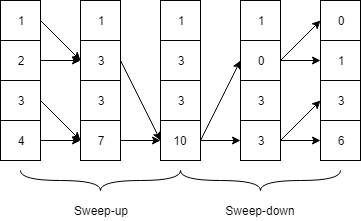
\includegraphics[width=0.5\linewidth]{Chapters/GPU/Algorithms/Belloch.png} 
    \caption{G. E. Belloch algorithm - exclusive scan}
\end{figure}


\subsection{Multiway partitioning}\label{sec:MultiwayPartitioning}

% Nice http://camlunity.ru/swap/Library/Conflux/Algorithms%20and%20Data%20Structures/gpuqsort.pdf

The multiway partitioning consists to split an unsorted set of $N$ items in $d$ bins such that all the elements in the $i$th bucket are smaller than the $d$th pivot and greater than the $d-1$th pivot given $d-1$ sorted pivots in increasing order.

This problem has most of its applications in GPU sorting~\cite{cederman2008practical}. Arge et al. proposes a more in depth analysis of the complexity in comparison to the original paper and gets: $O(\frac{N}{PB} + \lceil \frac{d}{B} \rceil \log P + d \log B)$.

The idea is a quite natural. We divide the initial vector in subelements, where we launch our processes. Each processor counts the number of elements smaller/greater than its relative pivot. Then, we compute a general scan to know at which index we will be able to write without having conflicts, elements greater than one pivot must be placed after all the elements which are smaller.

\subsection{Selection}

Given an unordered set of size $N$ and an integer $k$ (with $1 \leq k \leq N$). The selection problem consists to find an item such that it is larger than exactly $k - 1$ elements.

The idea is quite similar to the $k$th sort. We perform a multiway partitioning on the inputs and recurse on the targeted subset. This leads to a complexity in $O(\frac{N}{PB} + \log PB ~ \log \frac{N}{P})$; note that it considers an optimal algorithm for sorting in PRAM model when there are less elements than the number of processors~\cite{arge2008fundamental}.

